\section{Parametric lines}

\begin{outcome}

\begin{enumerate}

\item[A.] Find the vector and parametric equations of a line.

\end{enumerate}
\end{outcome}

We can use the concept of vectors and points to find equations for arbitrary lines in $\R^n$, although in this section the focus will be on lines in $\R^3$. 

To begin, consider the case $n=1$ so we have $\R^{1}=\R$. There is only one line here which is the familiar number line, that is $\R$ itself. Therefore it is not necessary to explore the case of $n=1$ further. 

Now consider the case where $n=2$, in other words $\R^2$.  Let $P $ and $P_0$ be
two different points in $\R^{2}$ which are contained in a line
$L$. Let $\vect{p}$ and $\vect{p_0}$ be the position vectors for the points $P$ and $P_0$
respectively. Suppose that $Q$ is an arbitrary point on $L$. Consider the following
diagram.

\begin{center}
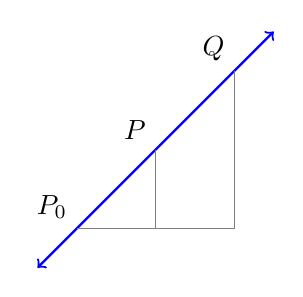
\begin{tikzpicture}
\draw[<->,thick,blue](-0.5,-0.5)--(2.5,2.5);
\draw[help lines](0,0)--(1,0)--(1,1);
\draw[help lines](0,0)--(2,0)--(2,2);
\node[above left] at (0,0){$P_0$};
\node[above left] at (1,1){$P$};
\node[above left] at (2,2){$Q$};
\end{tikzpicture}
\end{center}

Our goal is to be able to define $Q$ in terms of $P$  and $P_0$. Consider the vector $\longvect{P_0P} = \vect{p} - \vect{p_0}$ which
has its tail at $P_0$ and point at $P$. If we add $\vect{p} - \vect{p_0}$ to the position vector $\vect{p_0}$ for $P_0$,  
the sum would be a vector with its point at $P$. 
In other words,
\begin{equation*}
\vect{p} = \vect{p_0} + (\vect{p} - \vect{p_0})
\end{equation*}

Now suppose we were to add $t(\vect{p} - \vect{p_0})$ to $\vect{p}$ where $t$ is some scalar.
You can see that by doing so, we could find a vector with its point at $Q$. In other words, we can find $t$ such that 
\begin{equation*}
\vect{q} = \vect{p_0} + t \left( \vect{p}- \vect{p_0}\right)
\end{equation*}

This equation determines the line $L$ in $\R^2$. In fact, it determines a line $L$ in $\R^n$. Consider the following definition.

\begin{definition}{Vector equation of a line}{vectorequationofline}
Suppose a line $L$ in $\R^{n}$ contains the two\index{lines!vector equation} different points $P$ and 
$P_0$. Let $\vect{p}$ and $\vect{p_0}$ be the position vectors of these two points, respectively.
Then, $L$ is the collection of points $Q$ which have the position vector $\vect{q}$ given by
\begin{equation*}
\vect{q}=\vect{p_0}+t\left( \vect{p}-\vect{p_0}\right)
\end{equation*}
where $t\in \R$. 

Let $\vect{d} = \vect{p} - \vect{p_0}$. Then $\vect{d}$ is the \textbf{direction vector for $L$}\index{direction vector} and the \textbf{vector equation} for $L$ is given by 
\begin{equation*}
\vect{p}=\vect{p_0}+t\vect{d}, t\in\R
\end{equation*}
\end{definition}

Note that this definition agrees with the usual notion of a
line in two dimensions and so this is consistent with earlier concepts. Consider now points in $\R^3$. If a point $P \in \R^3$ is given by $P = \left( x,y,z \right)$, $P_0 \in \R^3$ by $P_0 = \left( x_0, y_0, z_0 \right)$, then we can write
\begin{equation*}
\left[
\begin{array}{c}
x \\
y \\
z 
\end{array}
\right] = 
\left[
\begin{array}{c}
x_0 \\
y_0 \\
z_0 
\end{array}
\right]
+
t
\left[
\begin{array}{c}
a \\
b \\
c 
\end{array}
\right]
\end{equation*}
where $\vect{d} = \left[
\begin{array}{c}
a \\
b \\
c 
\end{array}
\right]$. This is the vector equation of $L$ written in \textbf{component form}\index{component form}.

The following theorem claims that such an equation is in fact a line. 

\begin{proposition}{Algebraic description of a straight line}{algebraicstraightline}
Let $\vect{a},\vect{b}\in \R^{n}$ with $\vect{b}\neq \vect{0}$. 
Then $\vect{x}=\vect{a}+t\vect{b},\; t\in \R$, is a
line.
\end{proposition}

\begin{proof}
Let $\vect{x_{1}}, \vect{x_{2}} \in \R^n$. 
Define $\vect{x_{1}}=\vect{a}$ and let $\vect{x_{2}}-\vect{x_{1}}=\vect{b}$.
Since $\vect{b} \neq \vect{0}$, it follows that $\vect{x_{2}}\neq \vect{x_{1}}.$ Then
$\vect{a}+t\vect{b}=\vect{x_{1}} + t\left( \vect{x_{2}}-\vect{x_{1}}\right) $. It follows that  
$\vect{x}=\vect{a}+t\vect{b}$ is a line containing the two different points 
$X_1$ and $X_2$ whose position vectors are given by $\vect{x}_1$ and $\vect{x}_2$ respectively. 
\end{proof}

We can use the above discussion to find the equation of a line when given two distinct points.
Consider the following example. 

\begin{example}{A line from two points}{linefromtwopoints}
Find a vector equation for the line through the points $P_0 = \left(
1,2,0\right) $ and $P = \left( 2,-4,6\right).$
\end{example}

\begin{solution}
We will use the definition of a line given above in Definition \ref{def:vectorequationofline} to write
this line in the form 
\begin{equation*}
\vect{q}=\vect{p_0}+t\left( \vect{p}-\vect{p_0}\right)
\end{equation*}
Let $\vect{q} = 
\begin{mymatrix}{c}
x \\
y \\
z
\end{mymatrix}
$. Then, we can find $\vect{p}$ and $\vect{p_0}$ by taking the position vectors of points $P$ and $P_0$ 
respectively. 
Then, 
\begin{equation*}
\vect{q}=\vect{p_0}+t\left( \vect{p}-\vect{p_0}\right)
\end{equation*}
can be written as
\begin{equation*}
\begin{mymatrix}{c}
x \\
y \\
z \\
\end{mymatrix}
 =
\begin{mymatrix}{c}
1 \\
2 \\
0
\end{mymatrix}
+
t
\begin{mymatrix}{r}
 1 \\
-6 \\
6  
\end{mymatrix},
\;t\in
\R
\end{equation*}
Here, the direction vector $
\begin{mymatrix}{r}
1 \\
-6 \\
6 
\end{mymatrix}
$
is obtained by $
\vect{p} - \vect{p_0} = 
\begin{mymatrix}{r}
2 \\
-4 \\
6
\end{mymatrix}
-
\begin{mymatrix}{r}
1 \\
2 \\
0
\end{mymatrix}
$
as indicated above in Definition \ref{def:vectorequationofline}.
\end{solution} 

Notice that in the above example we said that we found ``a'' vector
equation for the line, not ``the'' equation.  The reason for this
terminology is that there are infinitely many different vector 
equations for the same line. To see this, replace $t$ with another
parameter, say $3s.$ Then you obtain a different vector equation for the same
line because the same set of points is obtained.

In Example \ref{exa:linefromtwopoints}, the vector given by 
$\begin{mymatrix}{r}
 1 \\
-6 \\
6 
\end{mymatrix}$
is the direction vector defined in Definition \ref{def:vectorequationofline}.
If we know the direction vector of a line, as well as a point on the line,
we can find the vector equation. 

Consider the following example. 

\begin{example}{A line from a point and a direction vector}{linepointanddirectionvector}
Find a vector equation for the line which contains the point $P_0 = \left(
1,2,0\right) $ and has direction vector $\vect{d} = 
\begin{mymatrix}{c}
1 \\
2 \\
1
\end{mymatrix}
$
\end{example}

\begin{solution}
We will use Definition \ref{def:vectorequationofline} to write this line in the form 
$\vect{p}=\vect{p_0}+t\vect{d},\; t\in \R$. We are given the direction vector $\vect{d}$. 
In order to find $\vect{p_0}$, we can use the position vector of the point $P_0$. 
This is given by 
$\begin{mymatrix}{c}
1 \\
2 \\
0
\end{mymatrix}.
$
Letting $\vect{p}
=
\begin{mymatrix}{c}
 x \\
y \\
z
\end{mymatrix}
$,
the equation for the line is given by 
\begin{equation}
\begin{mymatrix}{c}
x \\
y \\
z
\end{mymatrix}
=
\begin{mymatrix}{c}
1 \\
2 \\
0
\end{mymatrix}
+ 
t
\begin{mymatrix}{c}
1 \\
2 \\
1
\end{mymatrix},
\;t\in
\R \label{vectoreqn}
\end{equation}
\end{solution}

We sometimes elect to write a line such as the one given in \ref{vectoreqn} in the form
\begin{equation}
\begin{array}{ll}
\left. \begin{array}{l}
x=1+t \\
y=2+2t \\
z=t 
\end{array} \right\} & 
\mbox{where} \; t\in \R 
\end{array}
\label{parameqn}
\end{equation}
This set of equations give the same information as \ref{vectoreqn}, and is called the \textbf{parametric equation of the line}. 

Consider the following definition. 

\begin{definition}{Parametric equation of a line}{parametricequation}
Let $L$ be a line in $\R^3$ which has direction vector $\vect{d} = \begin{mymatrix}{c}
a \\
b \\
c
\end{mymatrix}$
and goes through the point $P_0 = \left( x_0, y_0, z_0 \right)$.
Then, letting $t$ be a parameter, we can write $L$ as 
\begin{equation*}
\begin{array}{ll}
\left.
\begin{array}{c}
x = x_0 + ta \\
y = y_0 + tb \\
z = z_0 + tc
\end{array}
\right\} & 
\mbox{where} \; t\in \R 
\end{array}
\end{equation*}
This is called a \textbf{parametric equation}\index{lines!parametric equation} of the line $L$.
\end{definition}

You can verify that the form discussed following Example \ref{exa:linepointanddirectionvector} in equation  \ref{parameqn} is of the form
given in Definition \ref{def:parametricequation}.

There is one other form for a line which is useful, which is the \textbf{symmetric form}. 
Consider the line given by  \ref{parameqn}. You can
solve for the parameter $t$ to write
\begin{equation*}
\begin{array}{l}
t=x-1 \\
t=\frac{y-2}{2} \\
t=z
\end{array}
\end{equation*}
Therefore, 
\begin{equation*}
x-1=\frac{y-2}{2}=z
\end{equation*}
This is the \textbf{symmetric form} of the line.\index{lines!symmetric form}

In the following example, we look at how to take the equation of a line from symmetric form to 
parametric form.

\begin{example}{Change symmetric form to parametric form}{symmetrictoparametric}
Suppose the
\textbf{symmetric form of a line} is
\begin{equation*}
\frac{x-2}{3}=\frac{y-1}{2}=z+3
\end{equation*}
Write the line in parametric form as well as vector form.
\end{example}

\begin{solution}
We want to write this line in the form given by Definition \ref{def:parametricequation}. This is of the form 
\begin{equation*}
\begin{array}{ll}
\left.
\begin{array}{c}
x = x_0 + ta \\
y = y_0 + tb \\
z = z_0 + tc
\end{array}
\right\} & 
\mbox{where} \; t\in \R 
\end{array}
\end{equation*}

Let $t=\frac{x-2}{3},t=\frac{y-1}{2}$ and $t=z+3$, as given in the symmetric form of the line.
 Then solving for $x,y,z,$
yields
\begin{equation*}
\begin{array}{ll}
\left.
\begin{array}{c}
x=2 + 3t \\
y=1 + 2t \\
z=-3 + t 
\end{array}
\right\} & 
\mbox{with} \;t\in \R
\end{array}
\end{equation*}

This is the parametric equation for this line. 

Now, we want to write this line in the form given by Definition \ref{def:vectorequationofline}.
This is the form 
\begin{equation*}
\vect{p}=\vect{p_0}+t\vect{d}
\end{equation*}
where $t\in \R$.
This equation becomes
\begin{equation*}
\begin{mymatrix}{c}
x \\
y \\
z
\end{mymatrix} =
\begin{mymatrix}{r}
2 \\
1 \\
-3 
\end{mymatrix}
+
t
\begin{mymatrix}{r}
3 \\
2 \\
1 
\end{mymatrix},
\;t\in
\R
\end{equation*}
\end{solution}
